\documentclass[border=10pt]{standalone}
\usepackage{tikz}\usepackage{amsmath}\usetikzlibrary{arrows.meta,decorations.markings}
\begin{document}
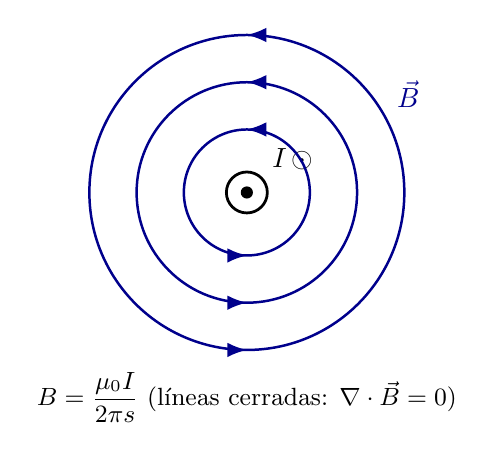
\begin{tikzpicture}[line width=0.9pt,>={Latex[length=2.2mm]}]
  % hilo saliente de la pagina
  \draw[line width=1pt] (0,0) circle(0.26);
  \fill (0,0) circle(2.2pt);
  \node at (0.58,0.42){$I\,\odot$};
  % lineas de B concentricas (antihorario para corriente saliente)
  \foreach \r in {0.8,1.4,2.0} \draw[blue!55!black,decoration={markings,mark=at position 0.25 with {\arrow{Latex}},mark=at position 0.75 with {\arrow{Latex}}},postaction={decorate}] (0,0) circle(\r);
  \node[blue!55!black] at (2.05,1.25){$\vec B$};
  \node at (0,-2.6){\small $\displaystyle B=\frac{\mu_0 I}{2\pi s}$ (líneas cerradas: $\nabla\cdot\vec B=0$)};
\end{tikzpicture}
\end{document}
